\title{Computational Genomics: Sequences \\
\large Homework 3
}
\author{
Srinivas Suresh
}
\date{\today}


\documentclass[12pt]{article}

\usepackage{enumitem}
\usepackage{algorithm}
\usepackage{algorithmic}
\usepackage{graphicx}
\usepackage{listings}
\usepackage{color}

\definecolor{dkgreen}{rgb}{0,0.6,0}
\definecolor{gray}{rgb}{0.5,0.5,0.5}
\definecolor{mauve}{rgb}{0.58,0,0.82}

\lstset{frame=tb,
language=Python,
aboveskip=3mm,
belowskip=3mm,
showstringspaces=false,
columns=flexible,
basicstyle={\small\ttfamily},
numbers=none,
numberstyle=\tiny\color{gray},
keywordstyle=\color{blue},
commentstyle=\color{dkgreen},
stringstyle=\color{mauve},
breaklines=true,
breakatwhitespace=true,
tabsize=3
}

\begin{document}
\maketitle

\section*{Answers}

\begin{enumerate}
\item answer1.py $>$ inputfile $<$ outputfile
\item answer2.py $>$ inputfile $<$ outputfile
\item 
\begin{enumerate}[label=(\alph*)]
        \item This is possible as sometimes you might end up replacing the character with itself
        \item This is also possible as everytime you might end up replacing the character with something other than itself
        \item This is not possible as you don't edit the list more than $n$ times
        
\end{enumerate}
\item  Completed tree below \\ 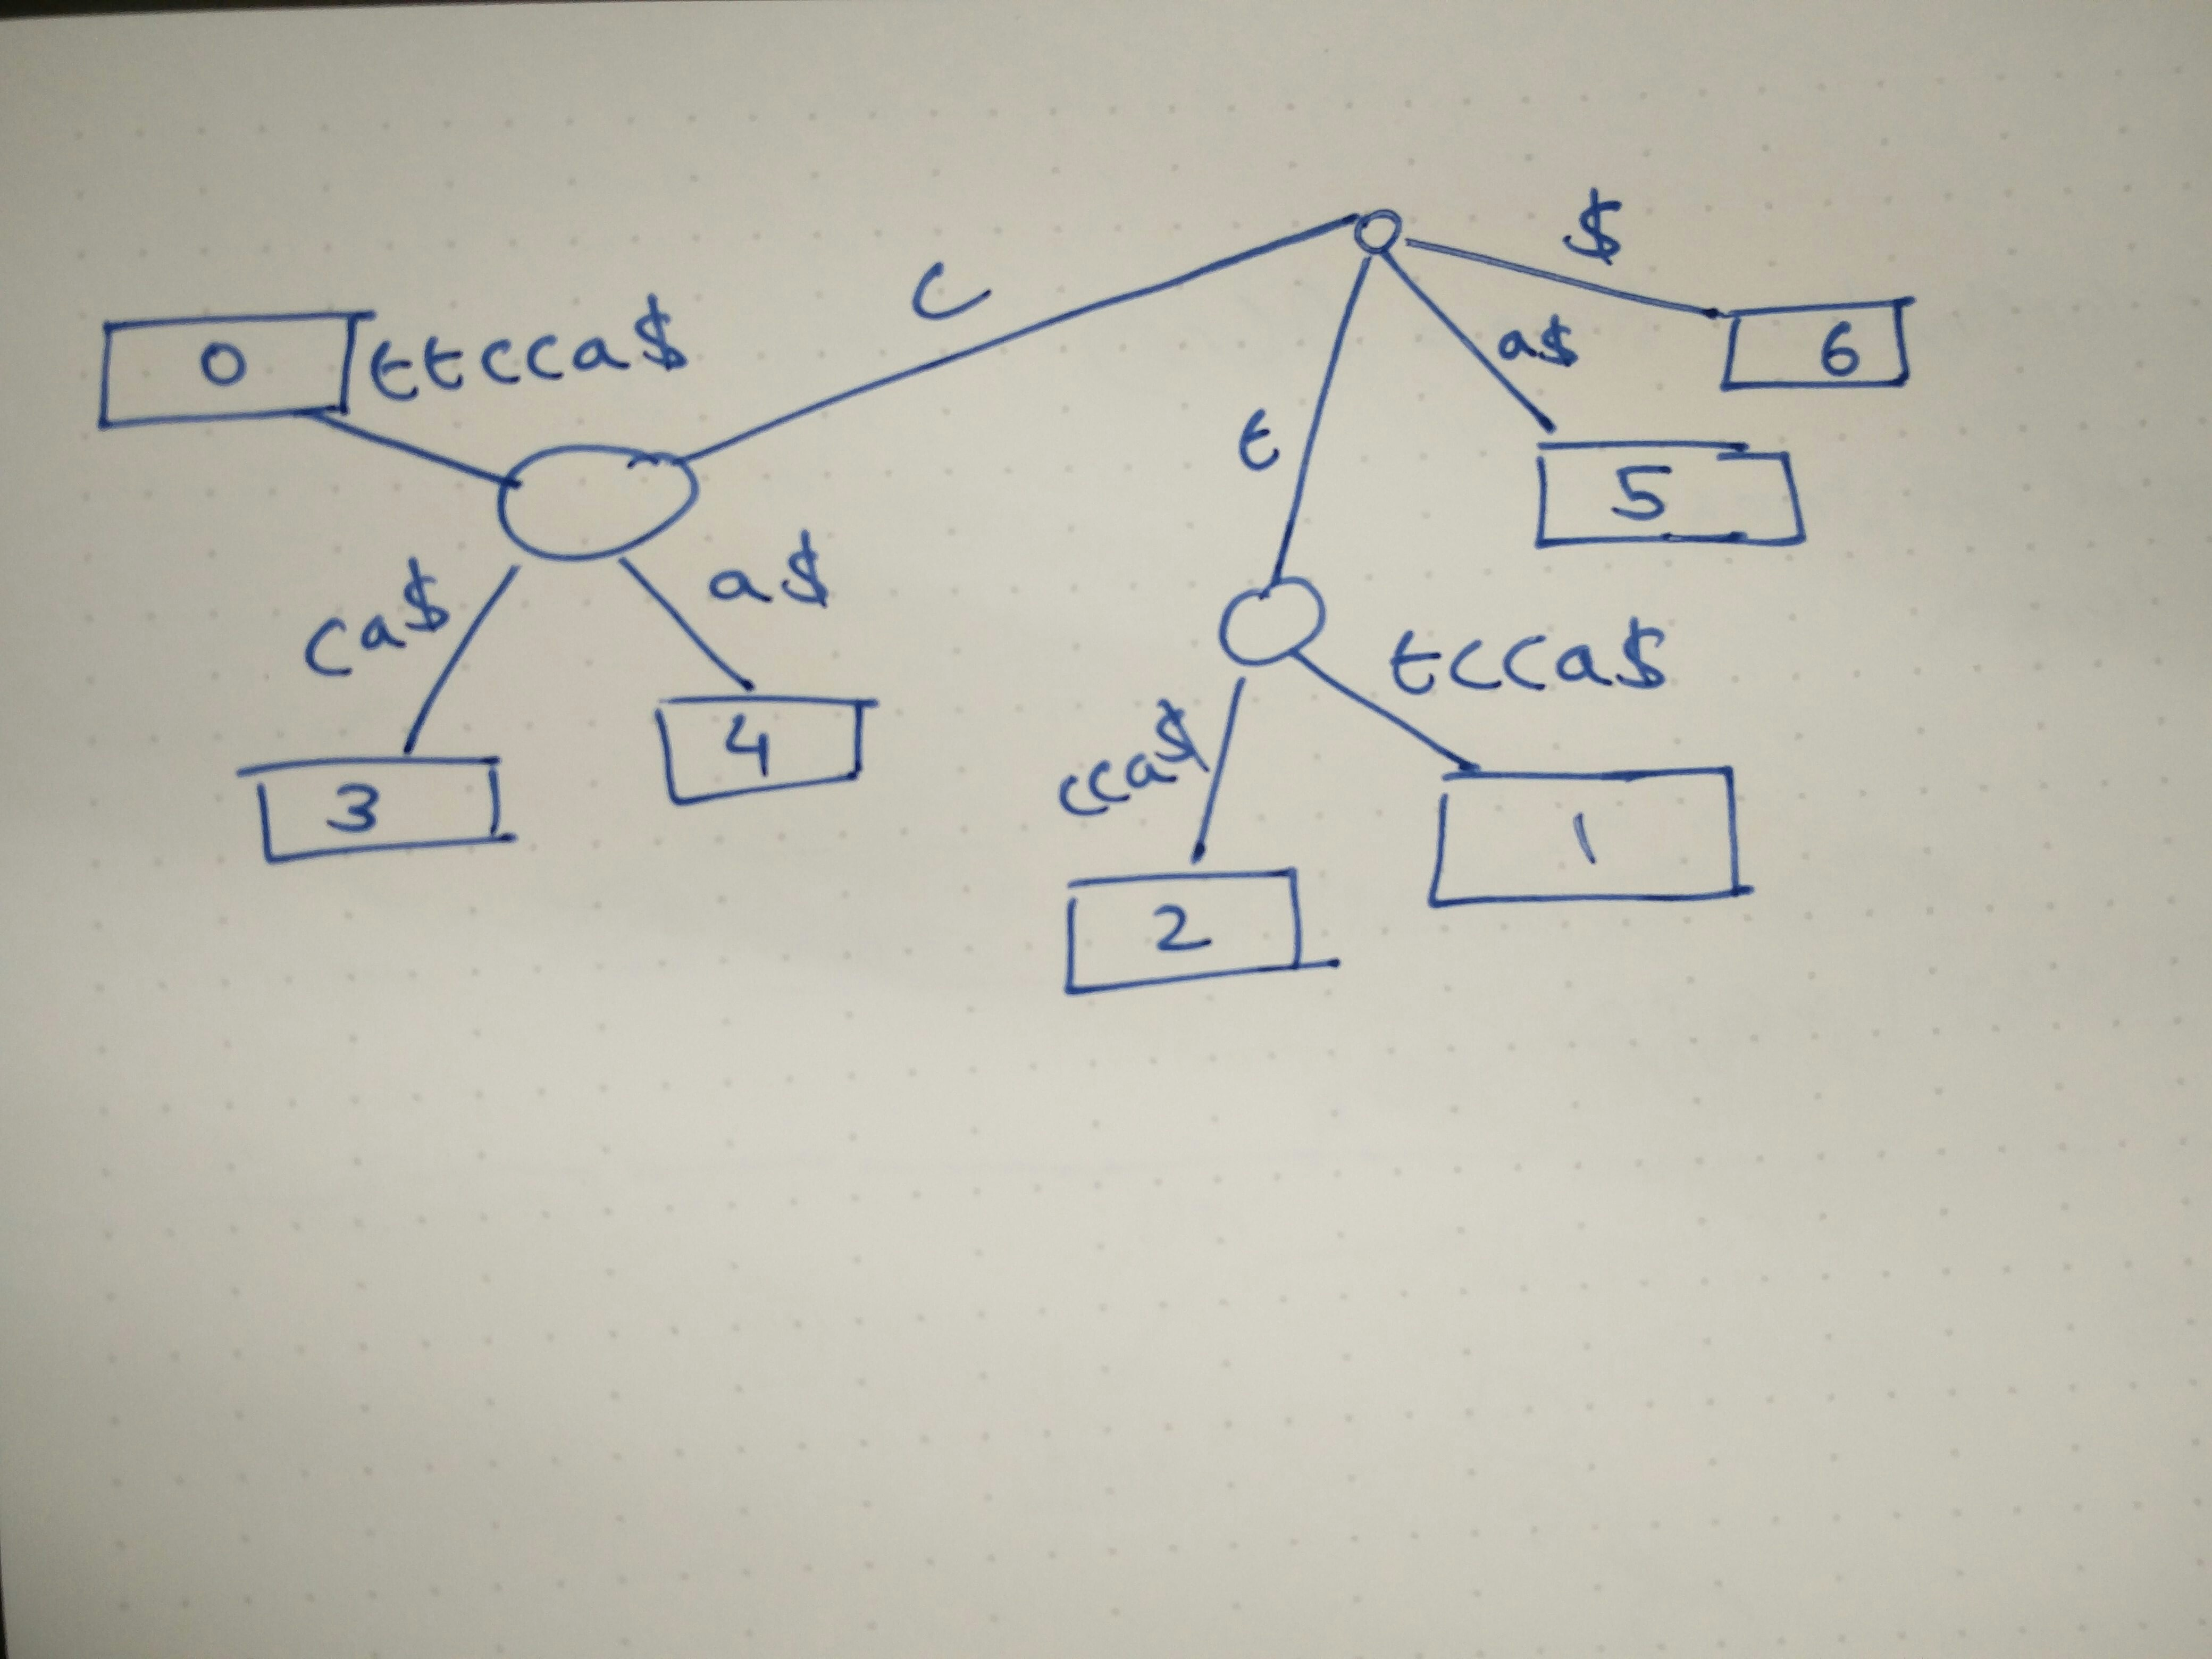
\includegraphics[scale=0.064]{4}
\item 
    \begin{enumerate}
        \item Below is the tree \\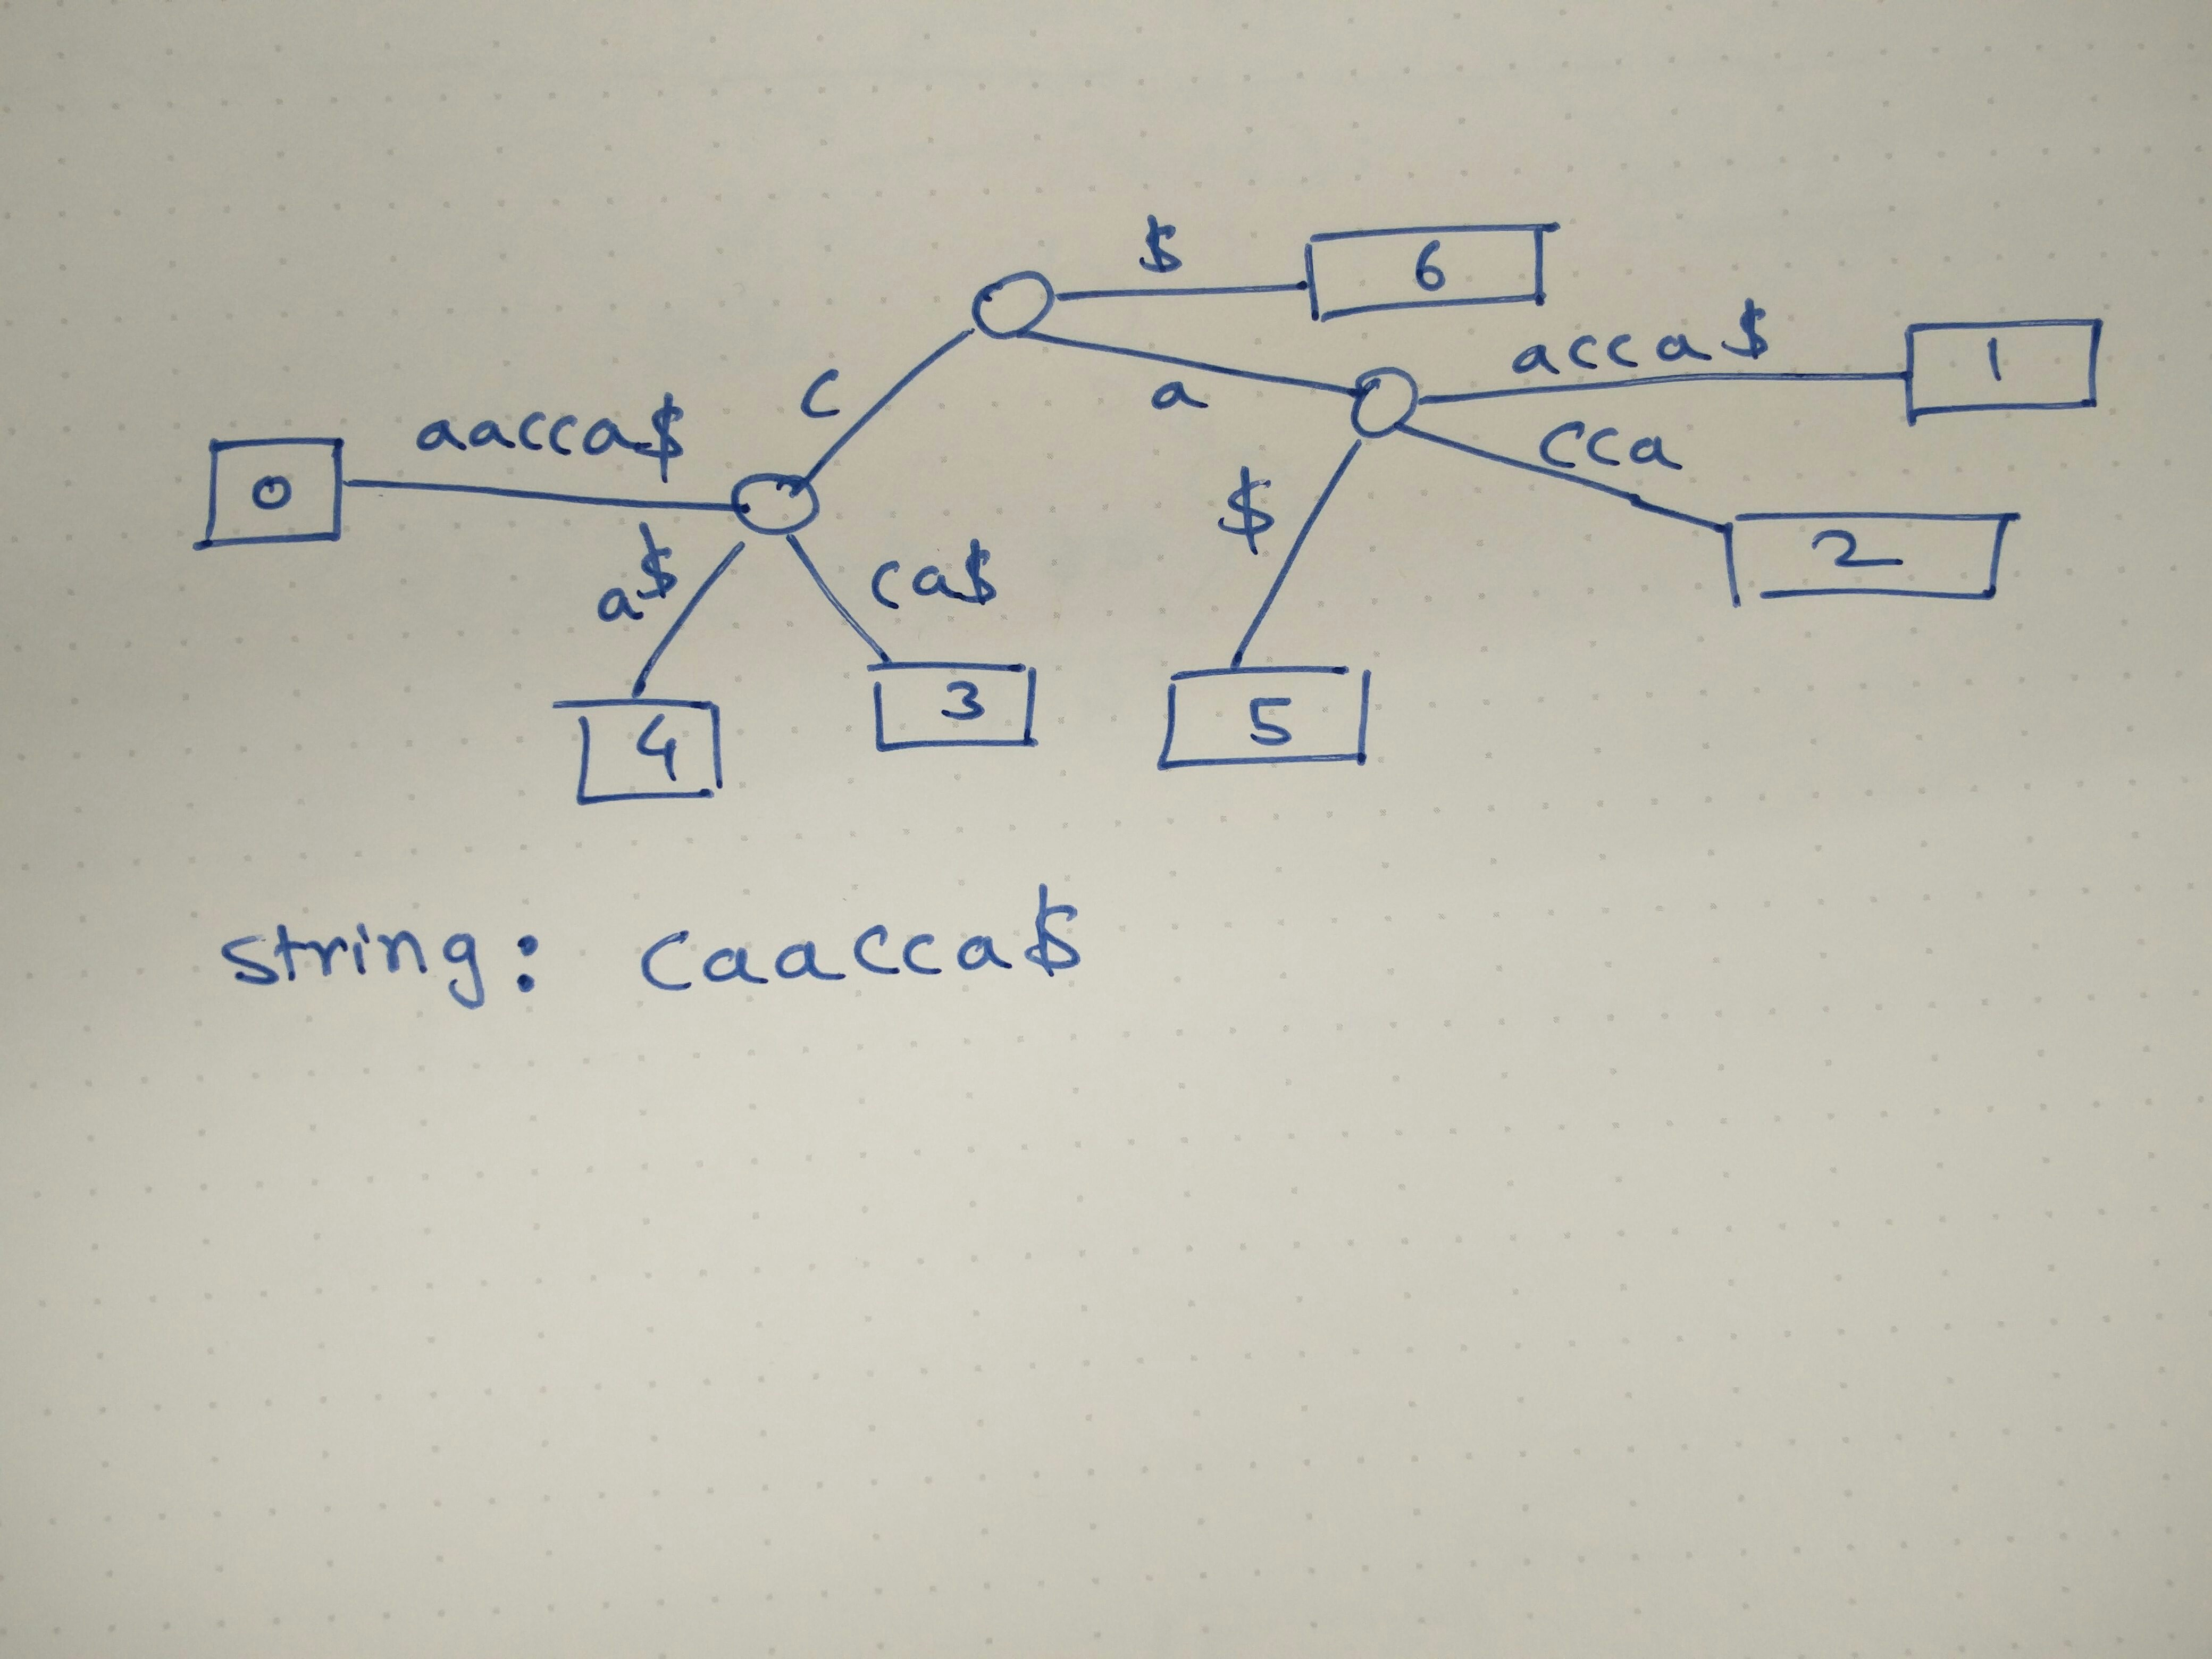
\includegraphics[scale=0.09]{5a}
        \item
            \begin{tabular}{ |c|c|c| } 
             \hline
             6 & \$\\
             5 & a\$\\
             1 & aacca\$\\
             2 & acca\$\\
             4 & ca\$\\
             0 & caacca\$\\
             3 & cca \$\\
             \hline
            \end{tabular}
        \item 
            lexicographically sorted rotations of $T$ \\
            \$CAACCA \\
            A\$CAACC \\
            AACCA\$C \\
            ACCA\$CA \\
            CA\$CAAC \\
            CAACCA\$ \\
            CCA\$CAA \\
            $BWT(T)$= ACCAC\$A
    \end{enumerate}
\item A string that has does not have contiguous chunks of repeating symbols would satisfy this requirement \\
    eg: $abcde\$$ . Would create a root node and a $\$$ node. And $m$ nodes representing the $m$ suffixes. Resulting in
     $m+2$ nodes.
\item
    \begin{enumerate}
        \item Construct 1 Generalized Suffix Tree for all the strings $O(N)$, separating each string with a unique terminal.
        \item Now we know that every string will have its own path in the suffix tree representing the string in its entireity
        \item We perform a DFS on the tree, visiting every node making note of the deepest node in terms of label depth
        for every string in the set of strings. We obtain pointers to these nodes and store them in a list: $O(N)$
        \item We iterate over this list and check if each of these nodes have a string other than the string they are
        the deeepest node for associated with them. If so then string for which this was the deepest node is a susbtring
        of another string.: $O(k)$
        \item Thus our algorithm works in linear time. This algorithm exploits the fact that \\
        \textbf{Every substring of a string is a prefix of some suffix}
    
    \end{enumerate}
\item The Burrows-Wheeler transform sorts the permuations by their \textit{right context}. This helps it brings similar/same characters together in 
“runs”. So, while storing, all characters need not be stored individually. One instance of a character along with the
number of times it occurs is sufficient. This helps in compression.
\item
    \begin{enumerate}
        \item Sorting the last column lexicographically will give you the first column of the matrix
        \item Yes. Every column between L and F are just permutations of the first column. so lexicographically Sorting
        would yield the first column
        \item The above hold for any row as well. Therfore this is still true.
    \end{enumerate}
    \pagebreak
\item 
    \begin{enumerate}
        \item There are multiple ways to solve this, but one way is shown below \\ 
             if $BWT(S)$ = A\textsubscript{0}A\textsubscript{1}C\textsubscript{0}G\textsubscript{0}G\textsubscript{1}G\textsubscript{2}\$
             \\ then, $F$ = \$A\textsubscript{0}A\textsubscript{1}C\textsubscript{0}G\textsubscript{0}G\textsubscript{1}G\textsubscript{2}
            \\ then, $S$ = G\textsubscript{2}G\textsubscript{1}G\textsubscript{0}C\textsubscript{0}A\textsubscript{1}A\textsubscript{0}\$
        \item \$GATGAG \\
        AG\$GATG \\
        ATGAG\$G \\
        G\$GATGA \\
        GAG\$GAT \\
        GATGAG\$ \\
        TGAG\$GA \\
    \end{enumerate}
\item $BWT(T)$ = C\textsubscript{0}C\textsubscript{1}T\textsubscript{0}\$A\textsubscript{0}G\textsubscript{0}G\textsubscript{1}\\
then, F = \$A\textsubscript{0}C\textsubscript{0}C\textsubscript{1}G\textsubscript{0}G\textsubscript{1}T\textsubscript{0}\\
then T\$ $\rightarrow$ C\textsubscript{1}A\textsubscript{0}G\textsubscript{0}G\textsubscript{1}T\textsubscript{0}C\textsubscript{0}\$
\item
    \begin{enumerate}
        \item $B$ ranked $BWT(T)$ \\
        \begin{tabular}{ |c|c|c| } 
            \hline
            \textbf{\$} & TTGAC & \textbf{A\textsubscript{0}}\\
            \textbf{A\textsubscript{0}} & \$TTGA & \textbf{C\textsubscript{0}}\\
            \textbf{A\textsubscript{1}} & CA\$TT & \textbf{G\textsubscript{0}}\\
            \textbf{C\textsubscript{0}} & A\$TTG & \textbf{A\textsubscript{1}}\\
            \textbf{G\textsubscript{0}} & ACA\$T & \textbf{T\textsubscript{0}}\\
            \textbf{T\textsubscript{0}} & GACA\$ & \textbf{T\textsubscript{1}}\\
            \textbf{T\textsubscript{1}} & TGACA & \textbf{\$}\\
            \hline
           \end{tabular} \\ \\
        Reversing to get $T$  \\
        \textbf{T\textsubscript{1}T\textsubscript{0}G\textsubscript{0}A\textsubscript{1}C\textsubscript{0}A\textsubscript{0}\$} \\
        
        \item In an \textit{LF} mapping, the i\textsuperscript{th} occurrence of a character in $F$ has the same rank 
        as the i\textsuperscript{th} occurrence of that character in $L$. Thanks to this property we can now reassign a rank based
        on the order of appearance of each character in either $F$ or $L$ as opposed to their order in $T$. This ranking is known
        as a \textit{B-ranking}. This sequential and ascending order of the ranks of the character greatly simplifies retrieval 
        of $T$ from the matrix
    \end{enumerate}

\end{enumerate}

\bibliographystyle{abbrv}
\bibliography{main}

\end{document}